\documentclass[UTF8]{ctexart}
\usepackage{CJKutf8}
\usepackage{graphicx}
\usepackage{subfig}
\usepackage{mathrsfs}
\usepackage{amsmath}
\usepackage{indentfirst}
\usepackage[colorlinks,linkcolor=red,anchorcolor=blue,citecolor=green]{hyperref}
\usepackage[linesnumbered,boxed,ruled,commentsnumbered]{algorithm2e}
\usepackage{cite}

  \author{黄晃\ 数院 1701210098 }
  \title{大数据项目二}
\begin{document}

  \maketitle
\section{问题}
使用Heat-Equatoin, Perona-Malik PDE进行去噪, 使用shock filters对图像进行去模糊.
  \section{算法}
\subsection{Heat-Equation}
$$ \left\{
\begin{aligned}
\frac{\partial u}{\partial t}&= \Delta u & t \geq 0, \\
u(0,x)& = u_0(x). &
\end{aligned}
\right.
$$
右端项使用简单的五点差分
\subsection{PM}
$$ \left\{
\begin{aligned}
\frac{\partial u}{\partial t}&= div(c(|\bigtriangledown u|^2) \Delta u), & t \geq 0, \\
u(0,x)& = u_0(x). &
\end{aligned}
\right.
$$
其中$c(s)=\frac{1}{1+s/K}$
\paragraph{$div(b\bigtriangledown u)$的计算}
使用非对称的离散格式,先计算各格点上的b的值,然后
$$
div(b\bigtriangledown u)=\frac{1}{h^2}(b_{i+1,j}u_{i+1,j}+b_{i,j}u_{i-1,j}+b_{i,j+1}u_{i,j+1}+b_{i,j}u_{i,j-1}-(b_{i+1,j}+b_{i.j+1}+2b_{i,j})v_{i,j})
$$
\subsection{shock filters}
$$ \left\{
\begin{aligned}
\frac{\partial u}{\partial t}&= -|\bigtriangledown u| F(\mathscr{L}(u)) & t \geq 0, \\
u(0,x)& = u_0(x). &
\end{aligned}
\right.
$$
其中$F(x)=x$, \\
$\mathscr{L}(u)=\Delta u\ ,or\ \frac{1}{|\bigtriangledown u|^2}(u_x^2u_{xx}+2u_xu_yu_{xy}+u_y^2u_{yy})$
\paragraph{$|\bigtriangledown u|$的逼近}
使用minmod算子
$$
m(a,b)=\left\{
\begin{aligned}
&sign(a)\min (|a|,|b|) & if\ ab>0 \\
&0 & if\ ab\leq 0
\end{aligned}
\right.
$$
$$
|\bigtriangledown u| = \frac{1}{h} \sqrt{m^2(\delta^+_xu,\delta_x^-u) + m^2(\delta^+_yu,\delta_y^-u)}
$$
\section{计算结果}
\paragraph{步长等参数的选取}
取$h=1,\Delta t = 0.05$,PM中$K=100$
\subsection{Heat Equation中时间T对处理结果的影响影响}
加了\%25的噪音,对T=1,2,5,10,20,50,100进行了测试,见图~\ref{fig:heat}.可以看到如下几点
\begin{itemize}
\item 随着T增大,图片噪声变小,但是T过大时,图片开始变得模糊

\end{itemize}
\begin{figure}
\subfloat[原图]{
\begin{minipage}[t]{0.3\linewidth}
\centering
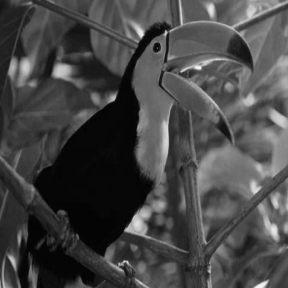
\includegraphics[width=1.5in]{./image_result/fig1.png}
\end{minipage}
}
\subfloat[noise]{
\begin{minipage}[t]{0.3\linewidth}
\centering
\includegraphics[width=1.5in]{./image_result/fig1_noise_heat.png}
\end{minipage}
}
\subfloat[T=1]{
\begin{minipage}[t]{0.3\linewidth}
\centering
\includegraphics[width=1.5in]{./image_result/fig1_result_heat_T1.png}
\end{minipage}
} 
\\
\subfloat[T=2]{
\begin{minipage}[t]{0.3\linewidth}
\centering
\includegraphics[width=1.5in]{./image_result/fig1_result_heat_T2.png}
\end{minipage}
}\subfloat[T=5]{
\begin{minipage}[t]{0.3\linewidth}
\centering
\includegraphics[width=1.5in]{./image_result/fig1_result_heat_T5.png}
\end{minipage}
}
\subfloat[T=10]{
\begin{minipage}[t]{0.3\linewidth}
\centering
\includegraphics[width=1.5in]{./image_result/fig1_result_heat_T10.png}
\end{minipage}
}
\\
\subfloat[T=20]{
\begin{minipage}[t]{0.3\linewidth}
\centering
\includegraphics[width=1.5in]{./image_result/fig1_result_heat_T20.png}
\end{minipage}
}
\subfloat[T=50]{
\begin{minipage}[t]{0.3\linewidth}
\centering
\includegraphics[width=1.5in]{./image_result/fig1_result_heat_T50.png}
\end{minipage}
}
\subfloat[T=100]{
\begin{minipage}[t]{0.3\linewidth}
\centering
\includegraphics[width=1.5in]{./image_result/fig1_result_heat_T100.png}
\end{minipage}
}
\caption{heat Equation}
\label{fig:heat}
\end{figure}

\subsection{PM方法结果}
设置与heat Eqaution中相同,结果见图~\ref{fig:pm}
\begin{itemize}
\item 随着T增大,图片噪声变小,但是T过大时,图片开始变得模糊
\item 整张图片的$\max (|\bigtriangledown u|)$随着T单调下降
\end{itemize}
\begin{figure}
\subfloat[原图]{
\begin{minipage}[t]{0.3\linewidth}
\centering
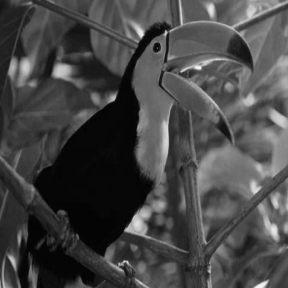
\includegraphics[width=1.5in]{./image_result/fig1.png}
\end{minipage}
}
\subfloat[noise]{
\begin{minipage}[t]{0.3\linewidth}
\centering
\includegraphics[width=1.5in]{./image_result/fig1_noise_pm.png}
\end{minipage}
}
\subfloat[T=1]{
\begin{minipage}[t]{0.3\linewidth}
\centering
\includegraphics[width=1.5in]{./image_result/fig1_result_pm_T1.png}
\end{minipage}
} 
\\
\subfloat[T=2]{
\begin{minipage}[t]{0.3\linewidth}
\centering
\includegraphics[width=1.5in]{./image_result/fig1_result_pm_T2.png}
\end{minipage}
}\subfloat[T=5]{
\begin{minipage}[t]{0.3\linewidth}
\centering
\includegraphics[width=1.5in]{./image_result/fig1_result_pm_T5.png}
\end{minipage}
}
\subfloat[T=10]{
\begin{minipage}[t]{0.3\linewidth}
\centering
\includegraphics[width=1.5in]{./image_result/fig1_result_pm_T10.png}
\end{minipage}
}
\\
\subfloat[T=20]{
\begin{minipage}[t]{0.3\linewidth}
\centering
\includegraphics[width=1.5in]{./image_result/fig1_result_pm_T20.png}
\end{minipage}
}
\subfloat[T=50]{
\begin{minipage}[t]{0.3\linewidth}
\centering
\includegraphics[width=1.5in]{./image_result/fig1_result_pm_T50.png}
\end{minipage}
}
\subfloat[T=100]{
\begin{minipage}[t]{0.3\linewidth}
\centering
\includegraphics[width=1.5in]{./image_result/fig1_result_pm_T100.png}
\end{minipage}
}
\caption{pm Equation}
\label{fig:pm}
\end{figure}


\subsection{shock filter的结果}
图片加上$\sigma=1.5$,kernel size=15的模糊,噪声分别为0.5\%,1\%,10\%.对于前面所给的两种L(以下称$\mathscr{L}=\Delta u$为mode1,否则为mode2)进行实验.具体为
\begin{itemize}
\item 取$\Delta t=0.05$,观察T=1,2,5,10时各个噪声的结果
\item 取$\Delta t=1$,观察T=100,1000,10000时噪声为1\%,0.5\%的结果
\end{itemize}
\begin{figure}
\subfloat[原图]{
\begin{minipage}[t]{0.3\linewidth}
\centering
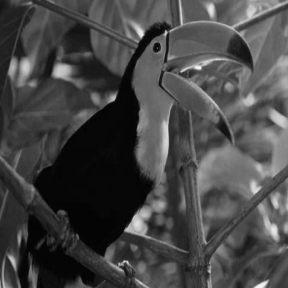
\includegraphics[width=1.5in]{./image_result/fig1.png}
\end{minipage}
}
\subfloat[noise]{
\begin{minipage}[t]{0.3\linewidth}
\centering
\includegraphics[width=1.5in]{./image_result/fig1_noise0005_shock.png}
\end{minipage}
}
\subfloat[T=1]{
\begin{minipage}[t]{0.3\linewidth}
\centering
\includegraphics[width=1.5in]{./image_result/fig1_result_shock0005mode1_T1.png}
\end{minipage}
} 
\\
\subfloat[T=2]{
\begin{minipage}[t]{0.3\linewidth}
\centering
\includegraphics[width=1.5in]{./image_result/fig1_result_shock0005mode1_T2.png}
\end{minipage}
}\subfloat[T=5]{
\begin{minipage}[t]{0.3\linewidth}
\centering
\includegraphics[width=1.5in]{./image_result/fig1_result_shock0005mode1_T5.png}
\end{minipage}
}
\subfloat[T=10]{
\begin{minipage}[t]{0.3\linewidth}
\centering
\includegraphics[width=1.5in]{./image_result/fig1_result_shock0005mode1_T10.png}
\end{minipage}
}

\caption{shock filter mode1, noise=0.5\%}
\label{fig:shock-short-mode1-noise0005}
\end{figure}

\begin{figure}
\subfloat[原图]{
\begin{minipage}[t]{0.3\linewidth}
\centering
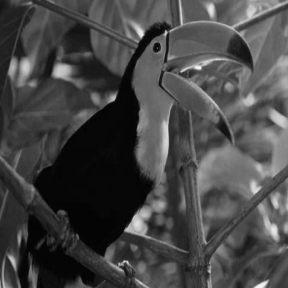
\includegraphics[width=1.5in]{./image_result/fig1.png}
\end{minipage}
}
\subfloat[noise]{
\begin{minipage}[t]{0.3\linewidth}
\centering
\includegraphics[width=1.5in]{./image_result/fig1_noise001_shock.png}
\end{minipage}
}
\subfloat[T=1]{
\begin{minipage}[t]{0.3\linewidth}
\centering
\includegraphics[width=1.5in]{./image_result/fig1_result_shock001mode1_T1.png}
\end{minipage}
} 
\\
\subfloat[T=2]{
\begin{minipage}[t]{0.3\linewidth}
\centering
\includegraphics[width=1.5in]{./image_result/fig1_result_shock001mode1_T2.png}
\end{minipage}
}\subfloat[T=5]{
\begin{minipage}[t]{0.3\linewidth}
\centering
\includegraphics[width=1.5in]{./image_result/fig1_result_shock001mode1_T5.png}
\end{minipage}
}
\subfloat[T=10]{
\begin{minipage}[t]{0.3\linewidth}
\centering
\includegraphics[width=1.5in]{./image_result/fig1_result_shock001mode1_T10.png}
\end{minipage}
}
\label{fig:shock-short-mode1-noise001}
\caption{shock filter mode1, noise=1\%}
\end{figure}

\begin{figure}
\subfloat[原图]{
\begin{minipage}[t]{0.3\linewidth}
\centering
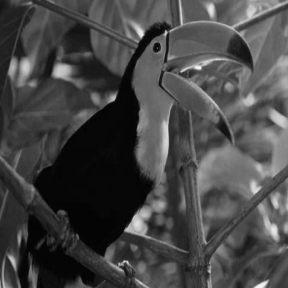
\includegraphics[width=1.5in]{./image_result/fig1.png}
\end{minipage}
}
\subfloat[noise]{
\begin{minipage}[t]{0.3\linewidth}
\centering
\includegraphics[width=1.5in]{./image_result/fig1_noise01_shock.png}
\end{minipage}
}
\subfloat[T=1]{
\begin{minipage}[t]{0.3\linewidth}
\centering
\includegraphics[width=1.5in]{./image_result/fig1_result_shock01mode1_T1.png}
\end{minipage}
} 
\\
\subfloat[T=2]{
\begin{minipage}[t]{0.3\linewidth}
\centering
\includegraphics[width=1.5in]{./image_result/fig1_result_shock01mode1_T2.png}
\end{minipage}
}\subfloat[T=5]{
\begin{minipage}[t]{0.3\linewidth}
\centering
\includegraphics[width=1.5in]{./image_result/fig1_result_shock01mode1_T5.png}
\end{minipage}
}
\subfloat[T=10]{
\begin{minipage}[t]{0.3\linewidth}
\centering
\includegraphics[width=1.5in]{./image_result/fig1_result_shock01mode1_T10.png}
\end{minipage}
}
\label{fig:shock-short-mode1-noise01}
\caption{shock filter mode1 ,noise=10\%}
\end{figure}

\begin{figure}
\subfloat[原图]{
\begin{minipage}[t]{0.3\linewidth}
\centering
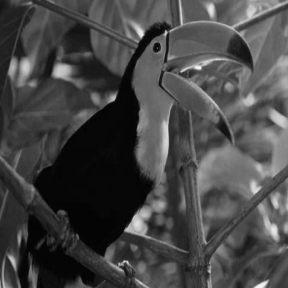
\includegraphics[width=1.5in]{./image_result/fig1.png}
\end{minipage}
}
\subfloat[noise]{
\begin{minipage}[t]{0.3\linewidth}
\centering
\includegraphics[width=1.5in]{./image_result/fig1_noise0005_shock.png}
\end{minipage}
}
\subfloat[T=1]{
\begin{minipage}[t]{0.3\linewidth}
\centering
\includegraphics[width=1.5in]{./image_result/fig1_result_shock0005mode2_T1.png}
\end{minipage}
} 
\\
\subfloat[T=2]{
\begin{minipage}[t]{0.3\linewidth}
\centering
\includegraphics[width=1.5in]{./image_result/fig1_result_shock0005mode2_T2.png}
\end{minipage}
}\subfloat[T=5]{
\begin{minipage}[t]{0.3\linewidth}
\centering
\includegraphics[width=1.5in]{./image_result/fig1_result_shock0005mode2_T5.png}
\end{minipage}
}
\subfloat[T=10]{
\begin{minipage}[t]{0.3\linewidth}
\centering
\includegraphics[width=1.5in]{./image_result/fig1_result_shock0005mode2_T10.png}
\end{minipage}
}

\caption{shock filter mode2, noise=0.5\%}
\label{fig:shockshortmode2noise0005}
\end{figure}

\begin{figure}
\subfloat[原图]{
\begin{minipage}[t]{0.3\linewidth}
\centering
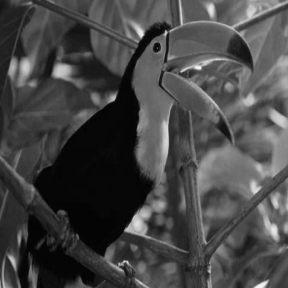
\includegraphics[width=1.5in]{./image_result/fig1.png}
\end{minipage}
}
\subfloat[noise]{
\begin{minipage}[t]{0.3\linewidth}
\centering
\includegraphics[width=1.5in]{./image_result/fig1_noise001_shock.png}
\end{minipage}
}
\subfloat[T=1]{
\begin{minipage}[t]{0.3\linewidth}
\centering
\includegraphics[width=1.5in]{./image_result/fig1_result_shock001mode2_T1.png}
\end{minipage}
} 
\\
\subfloat[T=2]{
\begin{minipage}[t]{0.3\linewidth}
\centering
\includegraphics[width=1.5in]{./image_result/fig1_result_shock001mode2_T2.png}
\end{minipage}
}\subfloat[T=5]{
\begin{minipage}[t]{0.3\linewidth}
\centering
\includegraphics[width=1.5in]{./image_result/fig1_result_shock001mode2_T5.png}
\end{minipage}
}
\subfloat[T=10]{
\begin{minipage}[t]{0.3\linewidth}
\centering
\includegraphics[width=1.5in]{./image_result/fig1_result_shock001mode2_T10.png}
\end{minipage}
}
\caption{shock filter mode2, noise=1\%}
\label{fig:shockshortmode2noise001}
\end{figure}

\begin{figure}
\subfloat[原图]{
\begin{minipage}[t]{0.3\linewidth}
\centering
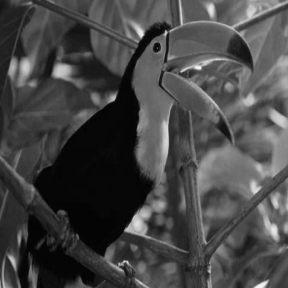
\includegraphics[width=1.5in]{./image_result/fig1.png}
\end{minipage}
}
\subfloat[noise]{
\begin{minipage}[t]{0.3\linewidth}
\centering
\includegraphics[width=1.5in]{./image_result/fig1_noise01_shock.png}
\end{minipage}
}
\subfloat[T=1]{
\begin{minipage}[t]{0.3\linewidth}
\centering
\includegraphics[width=1.5in]{./image_result/fig1_result_shock01mode2_T1.png}
\end{minipage}
} 
\\
\subfloat[T=2]{
\begin{minipage}[t]{0.3\linewidth}
\centering
\includegraphics[width=1.5in]{./image_result/fig1_result_shock01mode2_T2.png}
\end{minipage}
}\subfloat[T=5]{
\begin{minipage}[t]{0.3\linewidth}
\centering
\includegraphics[width=1.5in]{./image_result/fig1_result_shock01mode2_T5.png}
\end{minipage}
}
\subfloat[T=10]{
\begin{minipage}[t]{0.3\linewidth}
\centering
\includegraphics[width=1.5in]{./image_result/fig1_result_shock01mode2_T10.png}
\end{minipage}
}
\label{fig:shock-short-mode2-noise01}
\caption{shock filter mode2 ,noise=10\%}
\end{figure}

\begin{figure}
\subfloat[原图]{
\begin{minipage}[t]{0.3\linewidth}
\centering
\includegraphics[width=1.5in]{./image_result/fig1.png}
\end{minipage}
}
\subfloat[noise=10\%]{
\begin{minipage}[t]{0.3\linewidth}
\centering
\includegraphics[width=1.5in]{./image_result/fig1_noise01_shock.png}
\end{minipage}
}
\subfloat[mode2 moise=10\%]{
\begin{minipage}[t]{0.3\linewidth}
\centering
\includegraphics[width=1.5in]{./image_result/fig1_result_shock01mode2_T10000.png}
\end{minipage}
} 
\\
\subfloat[noise=1\%]{
\begin{minipage}[t]{0.3\linewidth}
\centering
\includegraphics[width=1.5in]{./image_result/fig1_noise001_shock.png}
\end{minipage}
}\subfloat[mode 1 noise = 1\%]{
\begin{minipage}[t]{0.3\linewidth}
\centering
\includegraphics[width=1.5in]{./image_result/fig1_result_shock001mode1_T10000.png}
\end{minipage}
}
\subfloat[mode 2 noise = 1\%]{
\begin{minipage}[t]{0.3\linewidth}
\centering
\includegraphics[width=1.5in]{./image_result/fig1_result_shock001mode2_T10000.png}
\end{minipage}
}
\\
\subfloat[noise=0.5\%]{
\begin{minipage}[t]{0.3\linewidth}
\centering
\includegraphics[width=1.5in]{./image_result/fig1_noise0005_shock.png}
\end{minipage}
}\subfloat[mode 1 noise = 0.5\%]{
\begin{minipage}[t]{0.3\linewidth}
\centering
\includegraphics[width=1.5in]{./image_result/fig1_result_shock0005mode1_T10000.png}
\end{minipage}
}
\subfloat[mode 2 noise = 0.5\%]{
\begin{minipage}[t]{0.3\linewidth}
\centering
\includegraphics[width=1.5in]{./image_result/fig1_result_shock0005mode2_T10000.png}
\end{minipage}
}
\caption{shock filter T=10000}
\label{fig:shocklong}

\end{figure}

\paragraph{shock filter结果的分析}
\begin{itemize}
\item mode2比mode1更稳定.在附加10\%的噪声时,设置时间步长为1,简单的使用$\mathscr{L}=\Delta u$s时,随着T的增大,会产生数值的溢出.相反,使用另一个$\mathscr{L}$仍然可以得到较好的结果
\item 在短时间内,噪音越大,则想恢复到相同的程度需要更大的T,比如图~\ref{fig:shockshortmode2noise0005} 和~\ref{fig:shockshortmode2noise001} 所显示的,0.5\%噪音下T=5已基本消去了噪声影响,而1\%噪声下需要T=10.而10\%噪声下,T=100时也仍存在肉眼可见的
\item 长时间下,T=10000时,10\%的噪声的结果已经不佳.
\item T=10000时,如图~\ref{fig:shocklong} 所示,由于相较于短时间,我们这里使用了更大的$\Delta t=1$,所以T=10000的结果比T=10的结果略有不如,具体表现在恢复结果对原光滑分界的破坏,不过仍有良好的效果.此外,虽然mode2有更好的稳定性,但是从图中可以看出,对于小的两个噪声,mode2的结果在分界线上产生了更多的尖刺.
\end{itemize}

\end{document} 
